\doublespacing
\setlength{\parindent}{1cm}

To understand Convolutional Neural Networks, we have to understand the following foundational ideas:

\begin{itemize}
  \item Convolution
  \item Pooling
  \item Jargon: padding, stride, filter, etc
\end{itemize}

In computer vision, we have used diverse techniques in the past on images to do object detection and image classification. One major problem with computer vision problems is that the input data can get really big. Suppose an image is of the size 68 X 68 X 3. The input feature dimension then becomes 12,288. This will be even bigger if we have larger images (say, of size 720 X 720 X 3). Now, if we feed this big input to a neural network, the number of parameters will swell up to a very large number (depending on the number of hidden layers and hidden units). This will result in more computational and memory requirements – not something most of us can deal with. \par

We begin by looking at edge detection as a simple example. The early layers of a neural network detect edges from an image. Deeper layers might be able to detect the cause of the objects and even more deeper layers might detect the cause of complete objects (like a person’s face). \par

\textbf{Edge Detection Problem}

In this section, we will focus on how the edges can be detected from an image. Suppose we are given the figure below:

\begin{figure}
  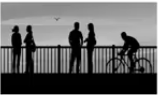
\includegraphics{edge-fig-1.png}
\end{figure}

As you can see, there are many vertical and horizontal edges in the image. Therefore, the first thing to be done is to detect these edges.

\begin{figure}
  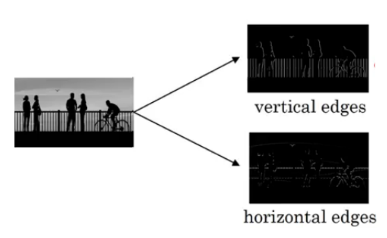
\includegraphics{edge-fig-2.png}
\end{figure}

How do we detect these edges? The first thing to do is assuming the image is BW, we represent it by a pixel map of gray scale values. Assume it is a 6 x 6 matrix.

\begin{figure}
  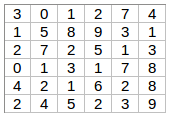
\includegraphics{matrix-fig-3.png}
\end{figure}

The values in these cells show pixel values in grayscale. Next, we convolve this 6 X 6 matrix with a 3 X 3 filter. They are also sometime referred to as feature detector or kernel.

\begin{figure}
  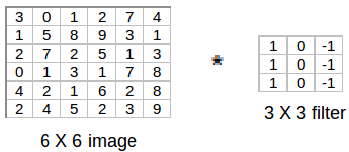
\includegraphics{mat-filter-fig-4.png}
\end{figure}

We take the feature filter and apply it over the original image. By placing it on the left upper corner, we get:

\begin{figure}
  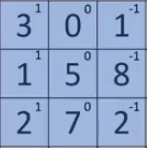
\includegraphics{mat-fig-5.png}
\end{figure}

So, we take the first 3 X 3 matrix from the 6 X 6 image and multiply it with the filter. Now, the first element of the output (which is a 4 X 4 matrix) will be the sum of the element-wise product of these values, i.e. 3*1 + 0 + 1*-1 + 1*1 + 5*0 + 8*-1 + 2*1 + 7*0 + 2*-1 = -5. To calculate the second element of the 4 X 4 output, we will shift our filter one step towards the right and again get the sum of the element-wise product:

\begin{figure}
  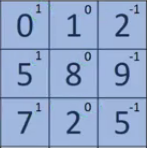
\includegraphics{mat-fig-6.png}
\end{figure}

Similarly, we will convolve over the entire image and get a 4 X 4 output:

\begin{figure}
  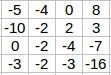
\includegraphics{mat-fig-7.png}
\end{figure}

The shifting of the filter is also called a stride. A stride of 1 shifts it one cell to the right, while a stride of 2 will shift it 2 cells to the right. So, convolving a 6 X 6 input with a 3 X 3 filter gave us an output of 4 X 4. This output is sometimes referred to as feature map. While the above explains what convolve operation does, we will take another example which can clarify how edges can be detected. If high pixel values represent bright areas and low values represent darker areas of an image, then look at this following example.

\begin{figure}
  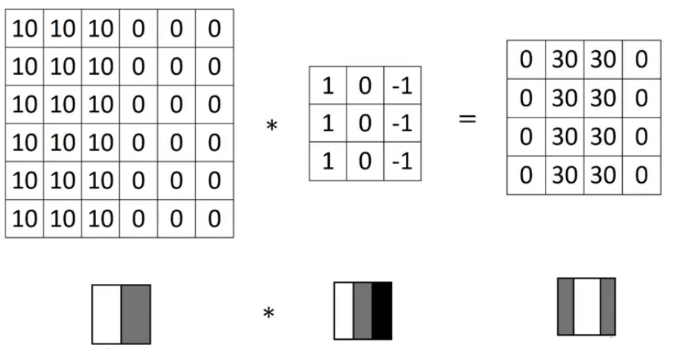
\includegraphics{conv-fig-8.png}
\end{figure}
